\documentclass[11pt,xcolor=dvipsnames]{beamer}
\usetheme{nelle}
\usepackage{natbib}                 % Fancy bibliography.
\usepackage{url}                    % Allow printing of URLs.
\usepackage{outlines}
\usepackage{enumitem}
\usepackage{multicol}
\usepackage{dsfont}
\usepackage{amsmath}
\usepackage{epstopdf}
\usepackage{color}
\usepackage[utf8]{inputenc}
\usepackage{tikz}
\usetikzlibrary{decorations.pathreplacing,positioning, arrows.meta}

\setbeamerfont{caption}{size=\scriptsize}
\setbeamertemplate{navigation symbols}{}
\setbeamertemplate{footline}{%
\hfill\usebeamertemplate***{navigation symbols}
\raisebox{2pt}[0pt][0pt]{%
\color{gray}\hspace{1cm} \insertframenumber{} }
}

\def\newblock{\hskip .11em plus .33em minus .07em}

\title{\textbf{Apprentissage statistique en haute dimension}\\
{\large Structures, régulation et fonction des génomes.}}
\subtitle{Candidature CR-CN en Section 07 au LIRIS (Team Beagle)}
\author[Varoquaux Nelle]{%
Nelle Varoquaux}
\date{28 Mars, 2019}
\institute{Department of Statistics, University of California, Berkeley}

\begin{document}
\begin{frame}[t, noframenumbering]
  \maketitle
\end{frame}

\setcounter{framenumber}{0}



\begin{frame}
\frametitle{Profile de recherche}

{\bf \small Un parcours interdisciplinaire}
\vskip-1.3ex
\rule{\dimexpr\paperwidth-1.5cm\relax}{0.4pt}
\begin{itemize}
\footnotesize
\item[-] Ingénieur Centrale Nantes (spécialité info), M2 MVA
\item[-] 2012-2015 Thèse à {\bf Mines ParisTech}, équipe CBIO (enc. J.-P. Vert)
\begin{itemize}
    \scriptsize
    \item[-] Analyse de la structure tri-dimensionnelle du génome à partir de
    données Hi-C
    \item[-] Étude de la structure tri-dimensionnelle du {\em P. falciparum}.
\end{itemize}
\item[-] 2016-2019 Postdoctorat à {\bf UC Berkeley} (enc. E. Purdom)
\begin{itemize}
    \scriptsize
    \item[-] Analyse fonctionnelle pour l'étude de
    données d'expression génique temporelles
    \item[-] Resistance à la sécheresse du sorgho.
\end{itemize}
\item[-] 2016-2018 Moore-Sloan Data Science fellow à BIDS
\begin{itemize}
    \scriptsize
    \item[-] Étude qualitative et quantitative des communautés du logiciel
    libre 
\end{itemize}
\end{itemize}

\vspace{1em}
{\bf \small Implication dans des grands consortiums}
\vskip-1.3ex
\rule{\dimexpr\paperwidth-1.5cm\relax}{0.4pt}
\begin{columns}
\begin{column}{0.2\linewidth}
\centering
\includegraphics[width=0.9\linewidth]{images/drought_wikipedia_square.png}
\end{column}
\begin{column}{0.8\linewidth}
\begin{itemize}[leftmargin=*]
\footnotesize
\item[-] \textbf{EPICON}\quad EPIgenetic CONtrol of drought resistance in sorghum
\begin{itemize}
\scriptsize
\item[-] 5 instituts de recherche, 8 équipes
\item[-] Étude de la dynamique de la réponse transcriptomique du sorgho sous
stresse de sécheresse.
{\tiny({\color{red}Varoquaux} et al., 2019)}
\end{itemize}
\item[-] \textbf{EMBER}\quad Exploring Maintainer Burnout through Ethnographic
Research
\begin{itemize}
\scriptsize
\item[-] 3 instituts de recherche
\item[-] Dynamique des communautés du logiciel libre ({\tiny Paxton,
{\color{red} Varoquaux} et al., (in preparation), Geiger, {\color{red}
Varoquaux} et al., 2018})
\end{itemize}
\end{itemize}
\end{column}
\end{columns}
\end{frame}

\begin{frame}
\frametitle{L'univers des données épigénétiques}
\begin{figure}
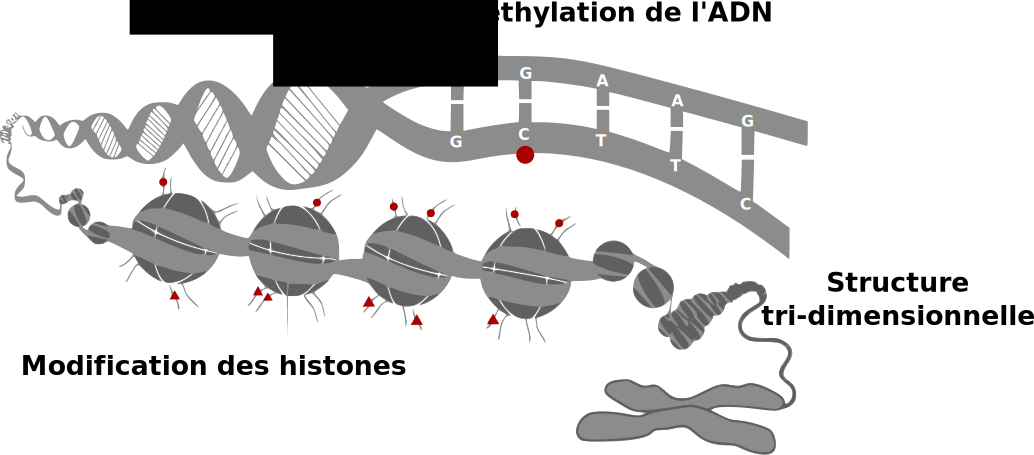
\includegraphics[width=0.8\linewidth]{images/dna-chromatin-histone.pdf}
\end{figure}
\begin{overlayarea}{12cm}{5cm}
\only<2>{
{\bf \small Les données épigénétiques : une vue multiple et globale sur la cellule}
\vskip-1.3ex
\rule{\dimexpr\paperwidth-1.5cm\relax}{0.4pt}
\begin{itemize}
\small
\item[-] Modification reversible de l'ADN ou de la chromatine; 
\item[-] Données hétérogènes permettant une vue multiple et
complète des médiateurs moléculaires.
\end{itemize}}
\only<3>{
{\bf \small Le défi de l'épigénétique}
\vskip-1.3ex
\rule{\dimexpr\paperwidth-1.5cm\relax}{0.4pt}
\begin{itemize}
\small
\item[-] Peu d'échantillons, beaucoup de descripteurs souvent corrélés ($n <
p$);
\item[-] Données larges, difficiles à manipuler;
\item[-] Données heteroscedastiques, bruitées, bruits de groupes;
\item[-] Modèle explicatif.
\end{itemize}
}

\end{overlayarea}

\end{frame}


\begin{frame}
\frametitle{Exemple I\quad Inférence de la structure 3D du génome}

\only<1>{%
\centering
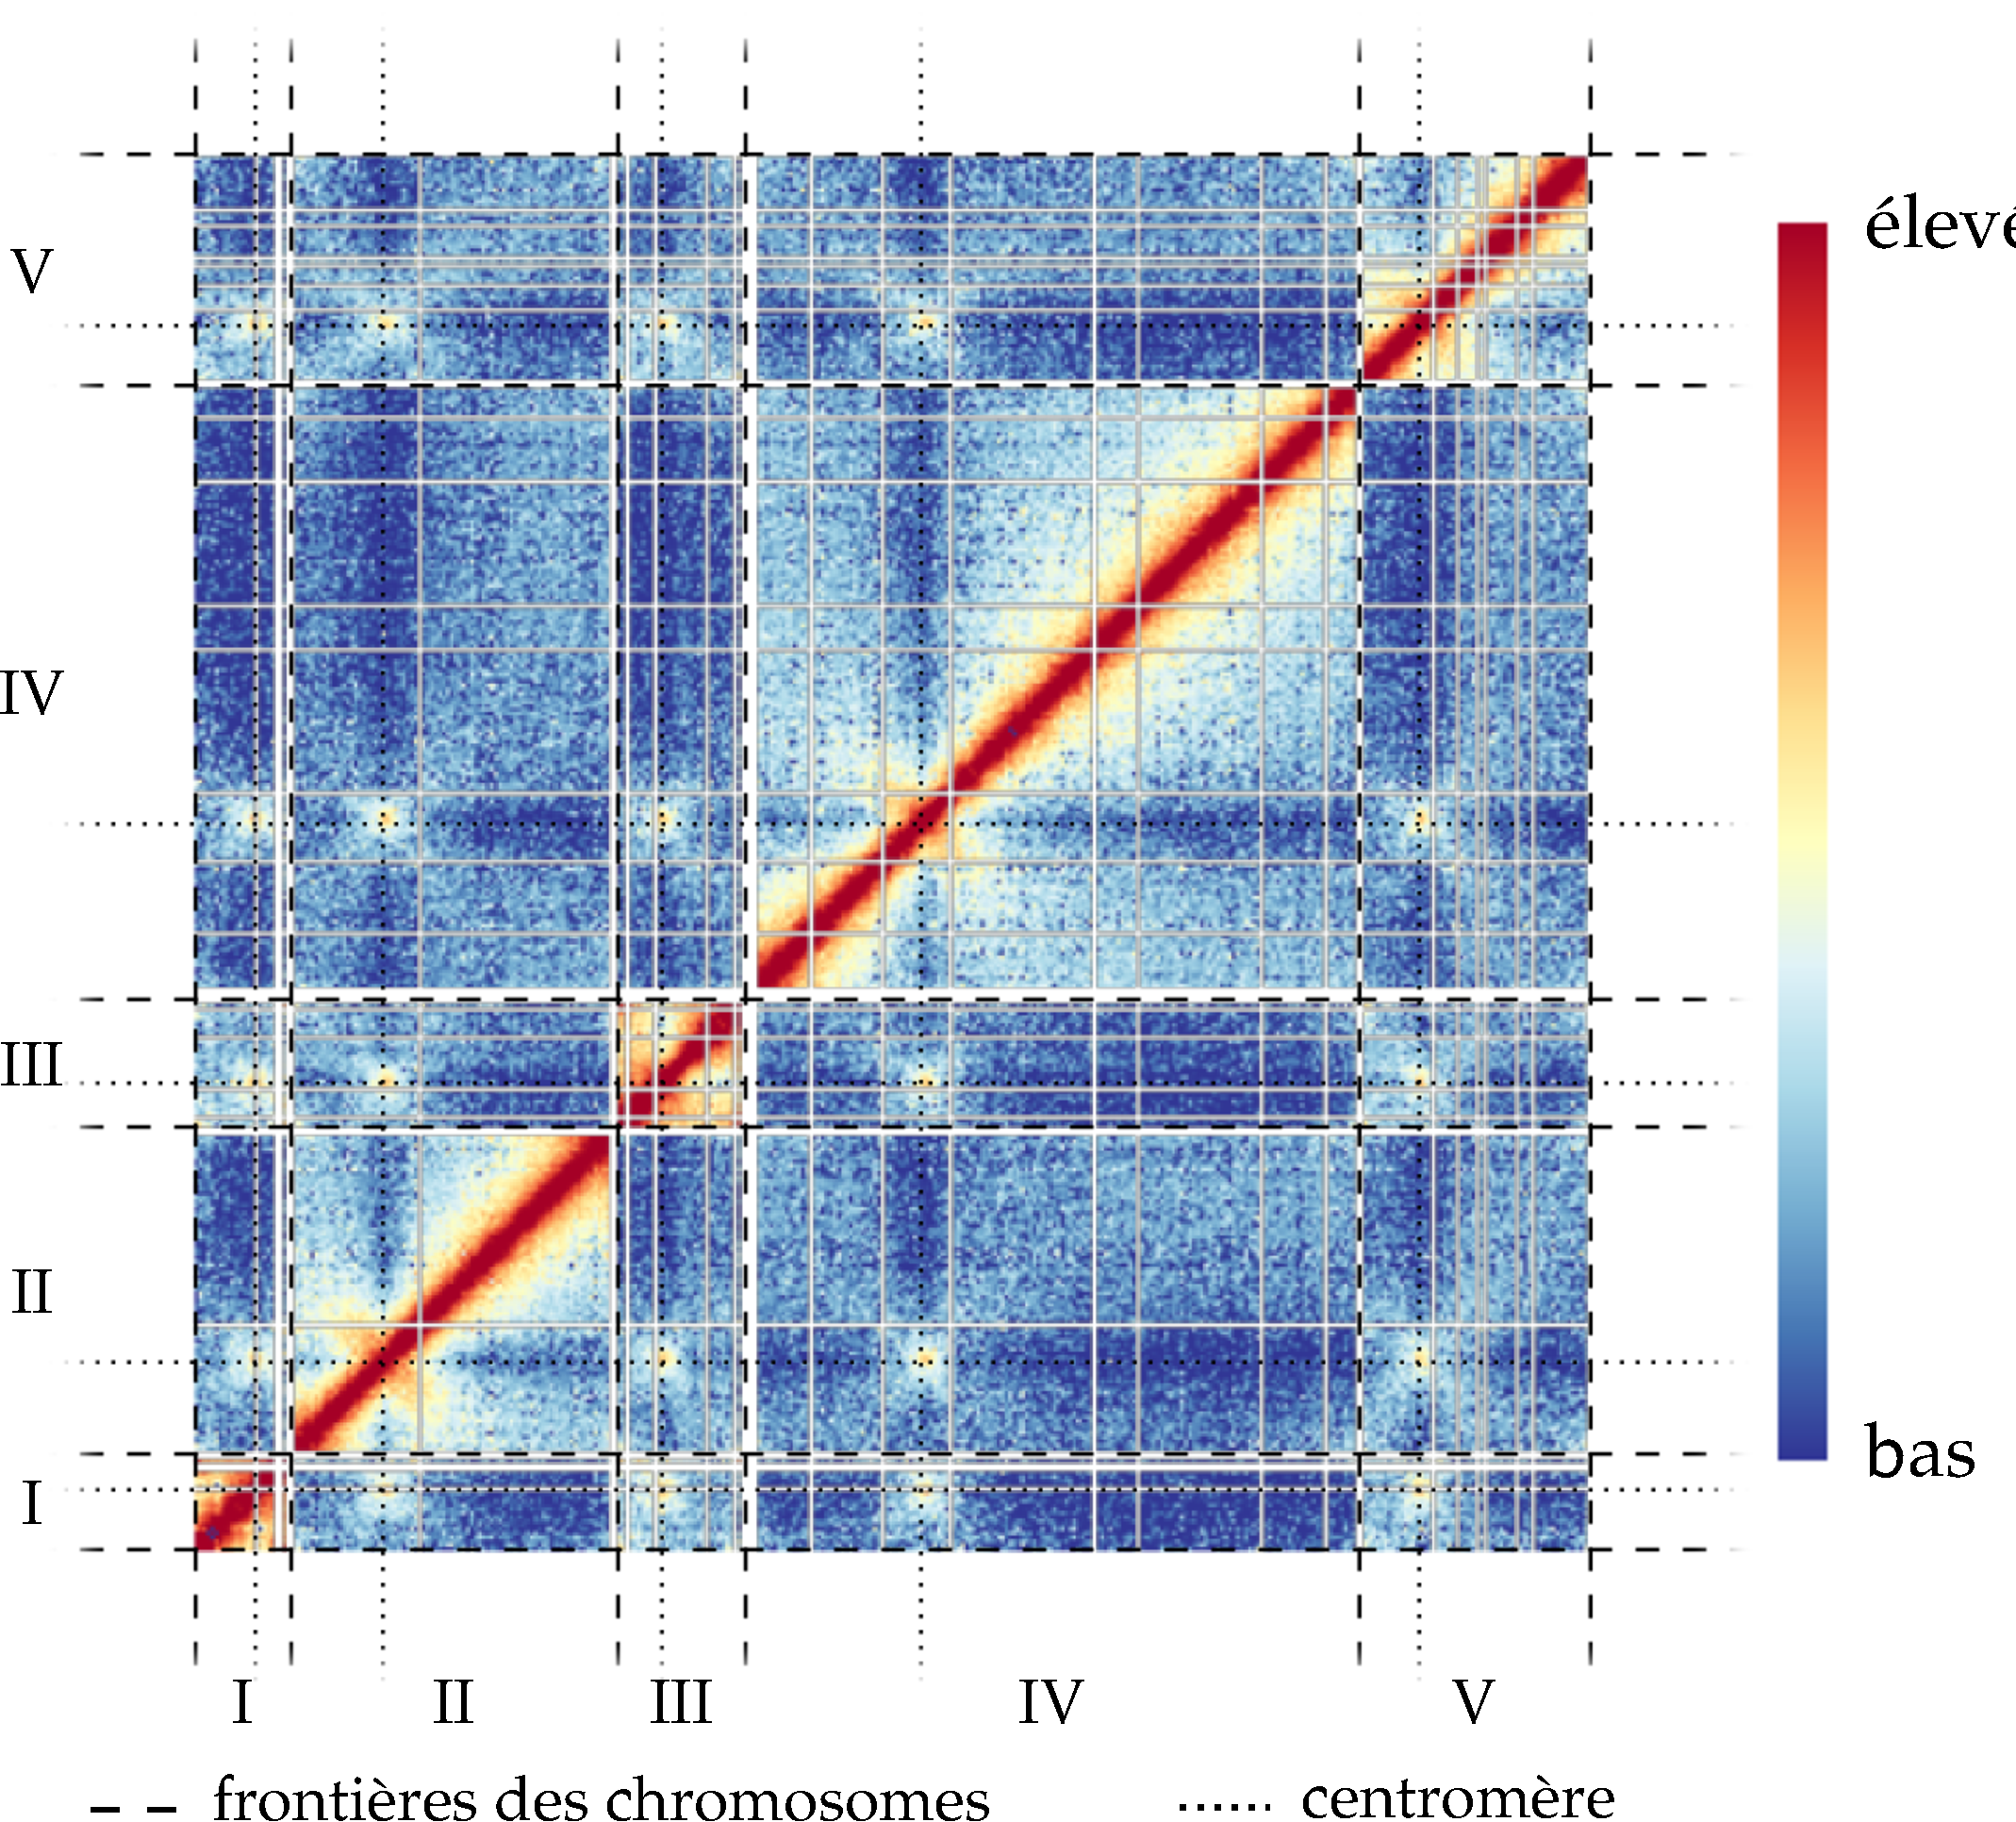
\includegraphics[width=0.6\linewidth]{figures/yeast_counts.pdf}
}

\begin{overlayarea}{12cm}{4cm}
\only<2->{%
\begin{center}
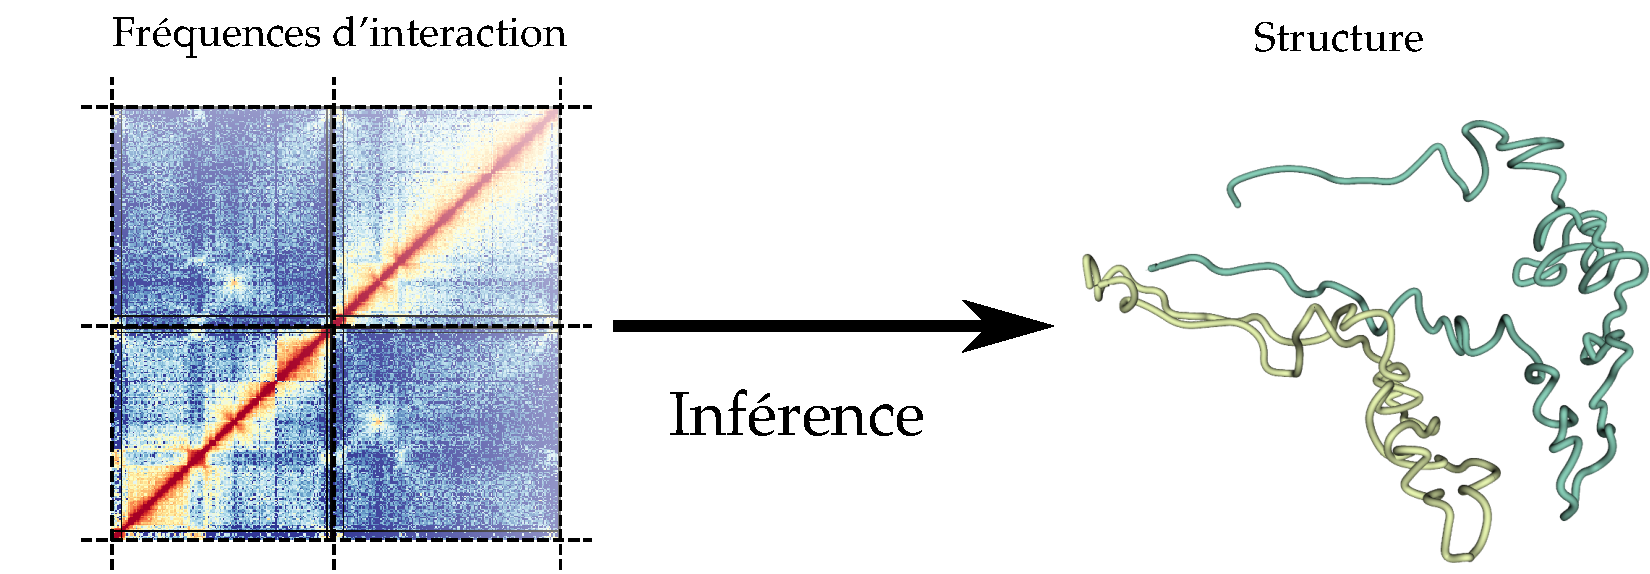
\includegraphics[width=0.9\linewidth]{figures/exemple_structure_inference.pdf}
\end{center}
}
\end{overlayarea}
\begin{overlayarea}{12cm}{4cm}
\only<3->{%
{\bf \small PASTIS}
\vskip-1.3ex
\rule{\dimexpr\paperwidth-1.5cm\relax}{0.4pt}
}

\only<3>{%
\begin{itemize}
\small
\item[-] Modélisation des chromosomes comme collier de $n$ perles
\item[-]
\begin{equation*}
\underbrace{c_{ij}}_{\text{\tiny fréquence d'interactions}} \sim
\quad
\text{Poisson}(\underbrace{\beta_{ij}}_{\text{\tiny bias}}
\underbrace{d_{ij}^\alpha}_{\text{\tiny distance}})
\end{equation*}
% FIXME rajouter à quoi correspondent les différents éléments de l'équation
\item[-] Maximization de la vraisemblance
\end{itemize}
}
\only<4>{%
\begin{itemize}
\small
\item[-] Modélisation des chromosomes comme collier de $n$ perles
\item[-]
\begin{equation*}
\underbrace{c_{ij}}_{\text{\tiny fréquence d'interactions}} \sim
\quad
\text{NB}(\underbrace{\beta_{ij}}_{\text{\tiny bias}}
\underbrace{d_{ij}^\alpha}_{\text{\tiny distance}},
\underbrace{\delta_{ij}}_{\text{\tiny dispersion}})
\end{equation*}
\item[-] Maximization de la vraisemblance
\end{itemize}
}
\only<3->{%
\begin{flushright}
{\tiny ({\color{red} Varoquaux} et al., 2014) ({\color{red} Varoquaux} et
al., In preparation)}
\end{flushright}
}
\end{overlayarea}
\end{frame}

\begin{frame}
\frametitle{Exemple II\quad Partionnement de données d'expression génique
temporelles}

\vspace{-2em}
\only<1>{%
\begin{figure}
\includegraphics[width=0.65\linewidth]{codes/images/splines_data.pdf}
\end{figure}}
\only<2>{%
\begin{figure}
\includegraphics[width=0.65\linewidth]{codes/images/splines_modeling.pdf}
\end{figure}}
\only<3>{%
\begin{figure}
\includegraphics[width=0.65\linewidth]{codes/images/gene_data.pdf}
\end{figure}}
\only<4->{%
\begin{figure}
\includegraphics[width=0.65\linewidth]{codes/images/scaled_centroids.pdf}
\end{figure}
}

\begin{overlayarea}{12cm}{5cm}
\only<5->{%
{\bf \small Partionnement via un modèle de mélange}
\vskip-1.3ex
\rule{\dimexpr\paperwidth-1.5cm\relax}{0.4pt}
}
\only<5>{%
\begin{equation*}
\underbrace{y_{ij}}_{\text{\tiny données}} \quad \sim \quad \sum_k \quad
\underbrace{\pi_k}_{\text{\tiny coefficient de mélange}}
\quad \mathcal{N}\large(a_{ik}\underbrace{\mu_k(t_j)}_{\text{\tiny centro\"ide}} +
b_{ik}, \sigma^2_{ikt}\large)
\end{equation*}
}
\only<6->{%
\begin{equation*}
\underbrace{y_{ij}}_{\text{\tiny données}} \quad \sim \quad \sum_k \quad
\underbrace{\pi_k}_{\text{\tiny coefficient de mélange}}
\quad \text{ZINB}\large(a_{ik}\underbrace{\mu_k(t_j)}_{\text{\tiny centro\"ide}} +
b_{ik} \large)
\end{equation*}
}
\vspace{-1.5em}
\only<5->{%
\begin{flushright}
\tiny ({\color{red} Varoquaux$^*$}, DeGraaf$^*$, Purdom, in preparation)
\end{flushright}
}

\end{overlayarea}

\end{frame}


\begin{frame}
\frametitle{Contributions principales}
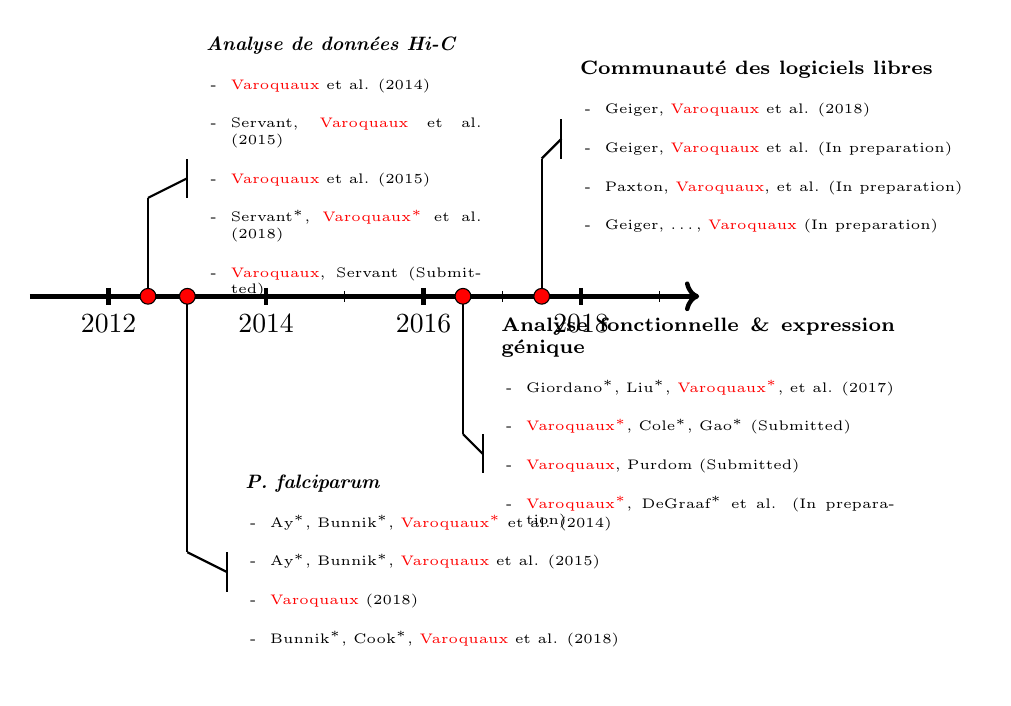
\begin{tikzpicture}

% Main horizontal line
\draw[ultra thick,->] (-1cm,0) -- (7.5,0);

% draw vertical lines
\foreach \x in {0,2,4,6}
    \draw[ultra thick] (\x cm,3pt) -- (\x cm,-3pt);
\foreach \x in {1,3,5,7}
    \draw (\x cm,2pt) --(\x cm,-2pt);

% draw names
\draw[ultra thick] (0,0) node[below=3pt,thick] {2012} node[above=3pt] {};
\draw[ultra thick] (2,0) node[below=3pt,thick] {2014} node[above=3pt] {};
\draw[ultra thick] (4,0) node[below=3pt, thick] {2016} node[above=3pt] {};
\draw[ultra thick] (6,0) node[below=3pt, thick] {2018} node[above=3pt] {};

% Hi-C
\draw [thick] (0.5 cm,2pt) -- (0.5cm,1.25cm);
\draw [fill=red](0.5,0) circle (0.1cm);
\draw [thick] (0.5cm,1.25cm) -- (1cm,1.5cm);
\draw [thick] (1cm,1.25cm) -- (1cm,1.75cm);
\draw [thick] (1cm, 1.5cm) node[right=3pt] {\parbox[t]{3.5cm}{\scriptsize {\bf
{\em Analyse de données Hi-C}}
\begin{itemize}[leftmargin=*]
\tiny
\item[-] {\color{red} Varoquaux} et al. (2014)
\item[-] Servant, {\color{red} Varoquaux} et al. (2015)
\item[-] {\color{red} Varoquaux} et al. (2015)
\item[-] Servant$^*$, {\color{red} Varoquaux$^*$} et al. (2018)
\item[-] {\color{red} Varoquaux}, Servant (Submitted)
\end{itemize}
}
};

% P. falciparum
\draw [thick] (1 cm,2pt) -- (1cm,-3.25cm);
\draw [fill=red](1,0) circle (0.1cm);
\draw [thick] (1cm,-3.25cm) -- (1.5cm,-3.5cm);
\draw [thick] (1.5cm,-3.25cm) -- (1.5cm,-3.75cm);
\draw [thick] (1.5cm, -3.5cm) node[right=3pt] {\parbox[t]{5cm}{\scriptsize {\bf
{\em P. falciparum}}
\begin{itemize}[leftmargin=*]
\tiny
\item[-] Ay$^*$, Bunnik$^*$, {\color{red} Varoquaux$^*$} et al. (2014)
\item[-] Ay$^*$, Bunnik$^*$, {\color{red} Varoquaux} et al. (2015)
\item[-] {\color{red} Varoquaux} (2018)
\item[-] Bunnik$^*$, Cook$^*$, {\color{red} Varoquaux} et al. (2018)
\end{itemize}
}
};

% EPICON
\draw [thick] (4.5 cm,2pt) -- (4.5cm,-1.75cm);
\draw [fill=red](4.5,0) circle (0.1cm);
\draw [thick] (4.5cm,-1.75cm) -- (4.75cm,-2cm);
\draw [thick] (4.75cm, -1.75cm) -- (4.75cm,-2.25cm);
\draw [thick] (4.75cm, -1.75cm) node[right=3pt] {\parbox[t]{5cm}{\scriptsize {\bf
Analyse fonctionnelle \& expression génique}
\begin{itemize}[leftmargin=*]
\tiny
\item[-] Giordano$^*$, Liu$^*$, {\color{red} Varoquaux$^*$}, et al. (2017)
\item[-] {\color{red} Varoquaux$^*$}, Cole$^*$, Gao$^*$ (Submitted)
\item[-] {\color{red} Varoquaux}, Purdom (Submitted)
\item[-] {\color{red} Varoquaux$^*$}, DeGraaf$^*$ et al. (In preparation) 
\end{itemize}
}
};

% EMBeR
\draw [thick] (5.5 cm,2pt) -- (5.5cm,1.75cm);
\draw [fill=red](5.5,0) circle (0.1cm);
\draw [thick] (5.5cm,1.75cm) -- (5.75cm,2cm);
\draw [thick] (5.75cm, 1.75cm) -- (5.75cm,2.25cm);
\draw [thick] (5.75cm, 1.75cm) node[right=3pt] {\parbox[t]{5cm}{\scriptsize {\bf
Communauté des logiciels libres}
\begin{itemize}[leftmargin=*]
\tiny
\item[-] Geiger, {\color{red} Varoquaux} et al. (2018)
\item[-] Geiger, {\color{red} Varoquaux} et al. (In preparation)
\item[-] Paxton, {\color{red} Varoquaux}, et al. (In preparation) 
\item[-] Geiger, \dots, {\color{red} Varoquaux} (In preparation) 
\end{itemize}
}
};

\end{tikzpicture}
\end{frame}

\begin{frame}
\frametitle{Projet de recherche}
\begin{center}
\em
Apprentissage statistique en haute-dimension: structures, fonctions et
régulation des génomes.
\end{center}

{\bf \small Analyse de la structure 3D du génome}
\vskip-1.3ex
\rule{\dimexpr\paperwidth-1.5cm\relax}{0.4pt}
\begin{itemize}
\small
\item[-] de populations homogènes
\item[-] de populations hétérogènes
\end{itemize}

\vspace{1em}
{\bf \small Inférence causale \& réseaux de régulations de
gènes}
\vskip-1.3ex
\rule{\dimexpr\paperwidth-1.5cm\relax}{0.4pt}
\begin{itemize}
\small
\item[-] Modélisation statique des médiateurs moléculaires
\item[-] Mise à l'échelle au génome entier : multi-tâches et régularisation 
\item[-] Modélisation dynamique pour des données longitudinales
\end{itemize}

\end{frame}

\begin{frame}
\frametitle{Analyse de la structure tri-dimensionelle du génome}

\begin{figure}
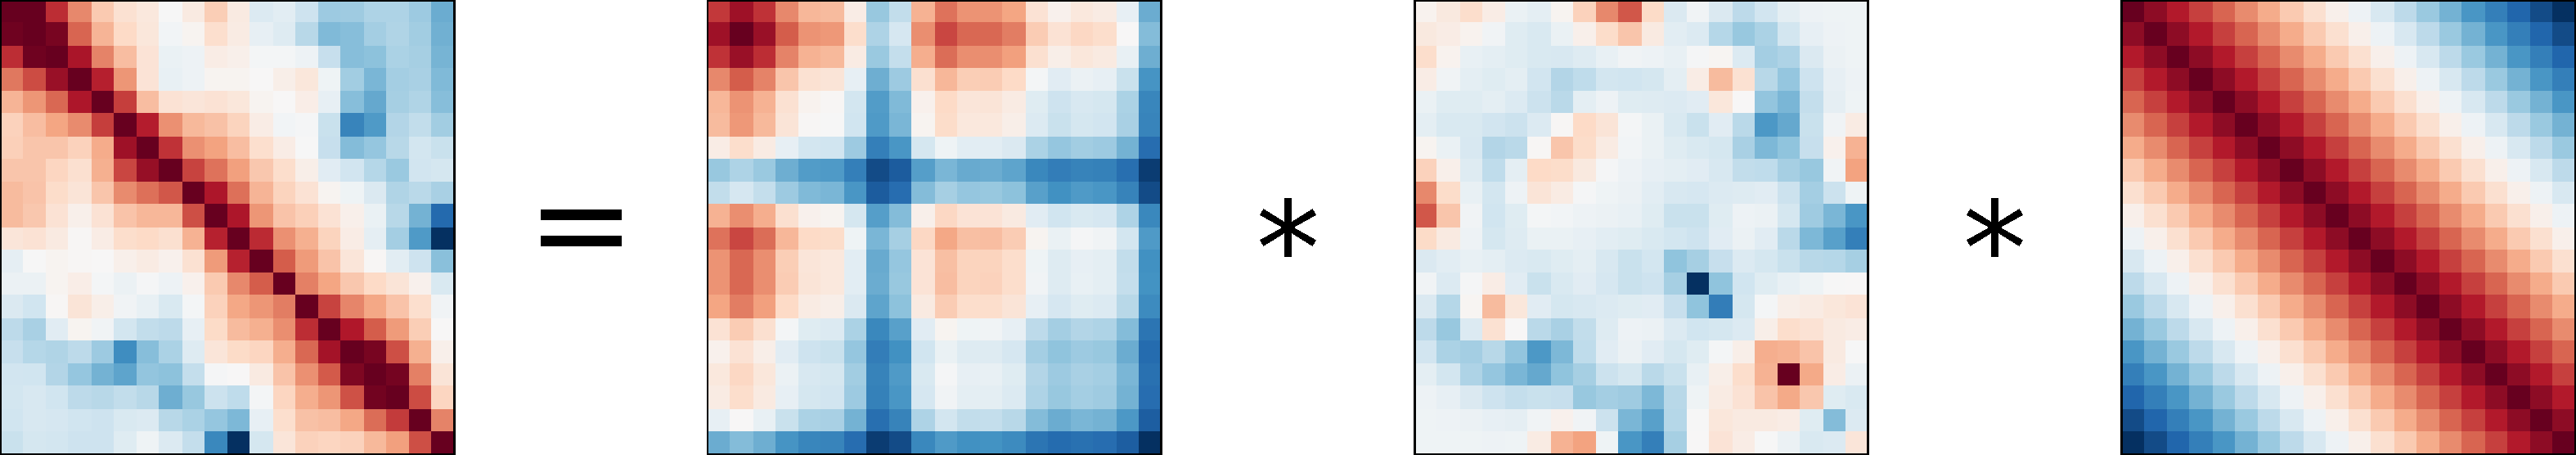
\includegraphics[width=0.7\linewidth]{figures/normalization.pdf}
\end{figure}
{\large
\begin{equation*}\label{eq:model} 
    \quad \quad \overbrace{\mathbb{E} c^k_{ij}} \quad = \quad
    \overbrace{\beta^k_i \beta^k_j} \quad * \quad
    \underbrace{\overbrace{(1+T^k_{ij})} \quad * \quad
    \overbrace{f^k(s(i,j))}}_{\text{\tiny Données normalisées}}\,,
\end{equation*}
}
{\small avec  $\sum_i c_{ij} = \sum f^k(s(i,j))$}

\vspace{1em}
\begin{overlayarea}{12cm}{4cm}
{\bf \small Une modélisation, quatre applications}
\vskip-1.3ex
\rule{\dimexpr\paperwidth-1.5cm\relax}{0.4pt}

\begin{itemize}
\footnotesize
\item[-] {\bf Normalisation au sein d'un échantillon}
\item[-] {\bf Normalisation across de plusieurs échantillons}, avec une
hypothèse supplémentaire sur la distribution marginale de $T^k_{ij}$
\item[-] {\bf Détection de pairs de loci d'interêt} via une pénalisation lasso
sur $T^k_{ij}$
\item[-] {\bf Analyse differentielle}, via des tests d'hypothèse sur
$T^k_{ij}$
\end{itemize}
\end{overlayarea}
\end{frame}

\begin{frame}
\frametitle{Inférence causale pour les réseaux de régulation de gènes}
\vspace{-0.5em}
\begin{columns}
\begin{column}{0.6\linewidth}
\begin{figure}
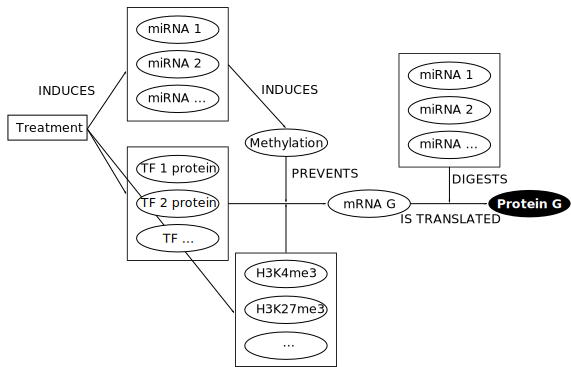
\includegraphics[width=\linewidth]{schemas/inferring_GRN.pdf}
\end{figure}
\end{column}
\begin{column}{0.35\linewidth}
\only<5->{%
\begin{center}
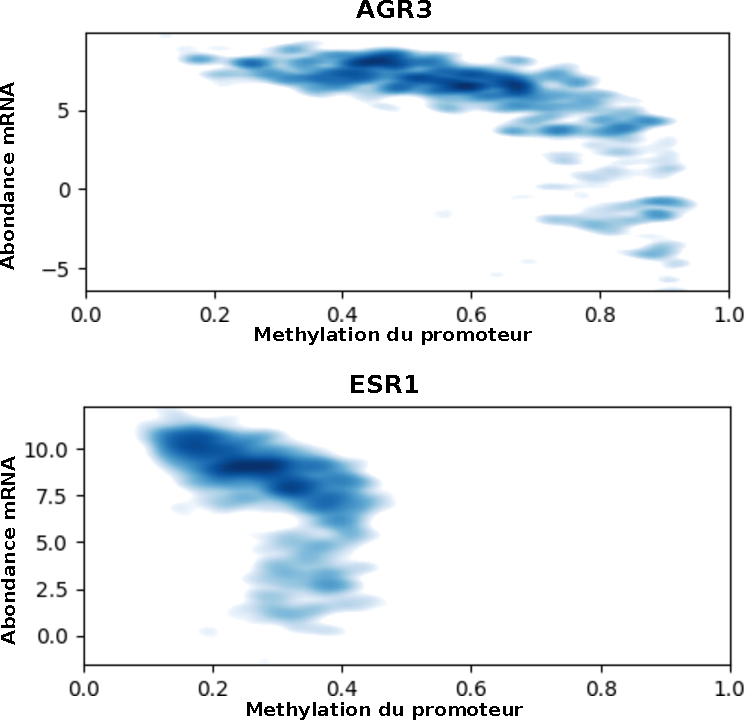
\includegraphics[width=\linewidth]{figures/methylation.pdf}
\end{center}
}
\end{column}
\end{columns}

\begin{overlayarea}{12cm}{4cm}
{\bf \small Modélisation statique des médiateurs moléculaires}
\vskip-1.3ex
\rule{\dimexpr\paperwidth-1.5cm\relax}{0.4pt}
\begin{columns}
\begin{column}{0.55\linewidth}
\only<2>{%
\begin{equation*}
y_G = f(\mathbf{X}_G)
\end{equation*}
}
\only<3->{%
\begin{align*}
y_G &= \beta^{\text{\tiny mRNA}}X^{\text{\tiny mRNA}}_G -
\beta^{\text{\tiny miRNA}}X^{\text{\tiny mRNA}}_G\\
X^{\text{\tiny mRNA}}_G &= f_{\text{\tiny methyl}}(X^{\text{\tiny methyl}})
f_{\text{\tiny HM}}(X^{\text{\tiny HM}})
(\beta^\text{\tiny TF}X^{\text{\tiny TF}}_G) \\
X^{\text{\tiny methy}}_G &= f_{\text{\tiny miRNA}}(X^{\text{\tiny
miRNA}})\\
\end{align*}
}
\end{column}
\begin{column}{0.45\linewidth}
\only<4->{
{\bf \footnotesize Défis}
\vskip-1.3ex
\rule{\dimexpr\linewidth-.5cm\relax}{0.4pt}
\begin{itemize}[leftmargin=*]
\scriptsize
\item[-] Nombre de médiateurs potentiels élevés; 
\item[-] Choix des descripteurs;
\item[-] Inférence de la forme des fonctions modératrices.
\end{itemize}}
\end{column}
\end{columns}
\end{overlayarea}
\end{frame}

\begin{frame}
\frametitle{Inférence causale pour les réseaux de régulation de gènes}
\vspace{-0.5em}
\begin{columns}
\begin{column}{0.6\linewidth}
\begin{figure}
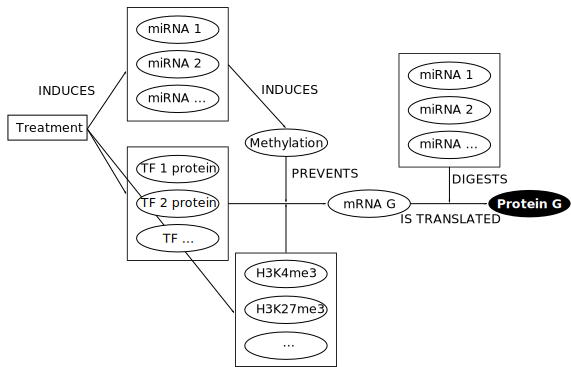
\includegraphics[width=\linewidth]{schemas/inferring_GRN.pdf}
\end{figure}
\end{column}
\begin{column}{0.35\linewidth}
\begin{center}
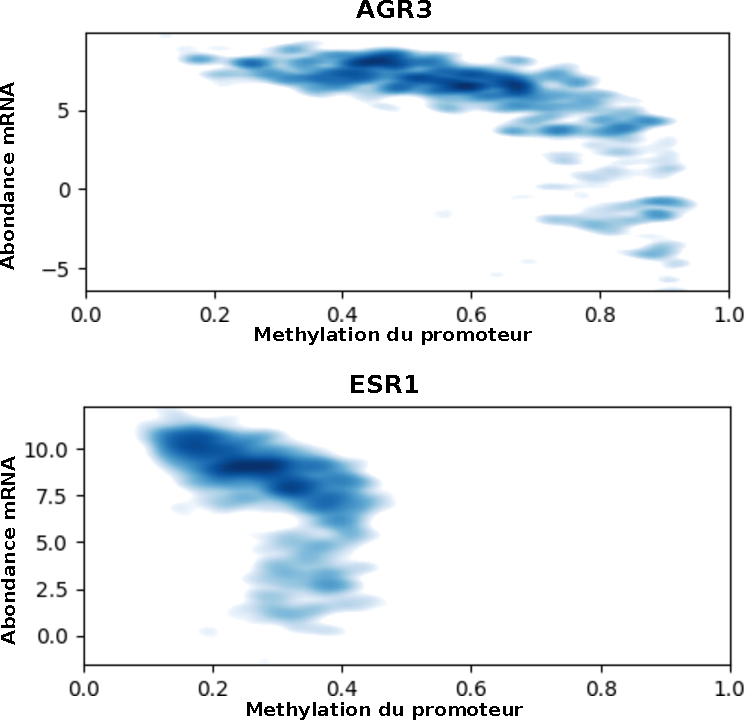
\includegraphics[width=\linewidth]{figures/methylation.pdf}
\end{center}
\end{column}
\end{columns}

\begin{overlayarea}{12cm}{4cm}
{\bf \small Mise à l'échelle au génome entier : multi-tâches et régularisation}
\vskip-1.3ex
\rule{\dimexpr\paperwidth-1.5cm\relax}{0.4pt}
\begin{itemize}
\footnotesize
\item[-] {\bf Défi}\quad 30,000 gènes chez l'humain;
\item[-] {\bf Stratégies proposées}
\begin{itemize}
\scriptsize
\item[-] Augmenter le nombre d'échantillon via d'autres jeux de données;
\item[-] Partage de l'information entre gènes;
\end{itemize}
\item[-] {\bf Solutions} \quad Exploiter les approches multi-tâches pour
partager les informations communes entre gènes et jeux de données;
\end{itemize}
\end{overlayarea}
\end{frame}


\begin{frame}
\frametitle{Résumé}
\begin{itemize}
\small
\item[-] {\em Profile de recherche}
\item[-] {\em Programme de recherche} \\
\begin{itemize}
\item Apprentissage statistique en haute dimension : structures,
régulations et fonction des génomes
\end{itemize}
\item[-] Adéquation avec les compétences du laboratoire d'accueil
\end{itemize}

\vspace{2em}
{\bf \small Production scientifique}
\vskip-1.3ex
\rule{\dimexpr\paperwidth-1.5cm\relax}{0.4pt}
\begin{itemize}
\small
\item[-] 10 publications de rang A dont 5 premier auteur, 2 deuxième auteur
\item[-] 2 publications soumises, 6 en cours de rédaction
\item[-] Contributions majeurs à 6 logiciels libres (dont
\texttt{scikit-learn}, \texttt{Matplotlib} et \texttt{scikit-image})
\end{itemize}
\end{frame}

\begin{frame}[t, noframenumbering]
\frametitle{Publications}

{\bf \small Publication de rang A, premier auteur}
\vskip-1.3ex
\rule{\dimexpr\paperwidth-1.5cm\relax}{0.4pt}
\begin{itemize}
\small
\item[-] Unfolding the Genome: The Case Study of {\em P. falciparum}. {\color{red}
Varoquaux} (2018)
\item[-] Effective normalization for copy number variation in Hi-C data.
Servant$^*$, {\color{red} Varoquaux$^*$} et al. (2018)
\item[-] Accurate identification of centromere locations in yeast genomes
using Hi-C. {\color{red} Varoquaux} et al. (2015)
\item[-] A statistical approach for inferring the 3D structure of the genome.
{\color{red} Varoquaux} (2014)
\item[-] Three-dimensional modeling of the P. falciparum genome during the
erythrocytic cycle reveals a strong connection between genome architecture and
gene expression. Ay, Bunnik, {\color{red} Varoquaux$^*$} et al. (2014)
\end{itemize}
\end{frame}

\begin{frame}[t, noframenumbering]
\frametitle{Publications}

{\bf \small Publication de rang A, deuxième auteur}
\vskip-1.3ex
\rule{\dimexpr\paperwidth-1.5cm\relax}{0.4pt}
\begin{itemize}
\small
\item[-] The Types, Roles, and Practices of Documentation in Data Analytics
Open Source Software Libraries. Geiger, {\color{red} Varoquaux} et al. (2018)
\item[-] HiC-Pro: an optimized and flexible pipeline for Hi-C data processing.
\quad Servant, {\color{red} Varoquaux} et al. (2015)
\end{itemize}

{\bf \small Autres publications de rang A}
\vskip-1.3ex
\rule{\dimexpr\paperwidth-1.5cm\relax}{0.4pt}
\begin{itemize}
\small
\item[-] Changes in genome organization of parasite-specific gene families
during the Plasmodium transmission stages. \quad Bunnik$^*$, Cook$^*$,
{\color{red} Varoquaux} et al. (2018)
\item[-] Identifying multi-locus chromatin contacts in human cells using
tethered multiple 3C. Ay, Vu, Zeitz, {\color{red} Varoquaux} (2015)
\item[-] A community effort to assess and improve drug sensitivity prediction
algorithms. Costello et al. (2014)
\end{itemize}
\end{frame}

\begin{frame}[t, noframenumbering]
\frametitle{Publications}

{\bf \small Publications soumises}
\vskip-1.3ex
\rule{\dimexpr\paperwidth-1.5cm\relax}{0.4pt}
\begin{itemize}
\item[-] Lifecycle transcriptomics of field-droughted sorghum reveals rapid
biotic and metabolic responses. \quad {\color{red} Varoquaux$^*$}, Cole$^*$,
Gao$^*$ et al. 
\item[-] FIXME pipeline paper 
\end{itemize}

{\bf \small Publications en cours de rédaction}
\vskip-1.3ex
\rule{\dimexpr\paperwidth-1.5cm\relax}{0.4pt}
\begin{itemize}
\item[-] jupyter
\item[-] documentation
\item[-] FOSS with Alex
\item[-] Clustering
\item[-] NB structure
\item[-] Diploid
\end{itemize}
\end{frame}

\begin{frame}[t, noframenumbering]
\frametitle{}
\end{frame}

\end{document}

